\documentclass{article}

\usepackage{graphicx}

\begin{document}
\section{Method}
\subsection{Participants}
Ten University of Connecticut undergraduate students participated, in partial fulfillment of a course requirement. Six participants were male and four female.

\subsection{Materials}
A wooden dowel 121.92~cm in length and 1.59~cm in diamter was used for dynamic-touch trials. A felt blindfold was used on dynamic-touch trials to eliminate visual information, and on visual trials while the experimenters adjusted the slope of the surface. Participants wore circumaural headphones playing white noise to eliminate auditory information while the experimenters adjusted the slope. Beeping noises were also played through the headphones to signal the start of each trial.  Participants indicated their responses by pressing a button on a Logitech wireless presentation remote. A PC running custom software written in Python controlled the audio and recorded participants' responses and response times.

\subsection{Apparatus}
The apparatus consisted of a solid wooden 75.88~cm x 210.19~cm platform leaned on a heavy metal block. The slope of the platform was adjusted by sliding the block along the floor. For seven angles of inclination---$12^\circ$, $17^\circ$, $22^\circ$, $27^\circ$, $33^\circ$, $39^\circ$, and $45^\circ$, the corresponding position of the block was determined and marked on the floor so it could be quickly recreated. The apparatus was strong and stable enough to support a person's weight. A rubber mat was attached to the platform in order to increase friction.

\subsection{Design and procedure}
The participant's task in this experiment was to determine whether a surface would support stable upright posture, defined as standing with feet flat and parallel without bending at the hip. With these restrictions, the slope can be accomodated primarily by bending at the ankle (Riccio \& Stoffregen, 1988). %\cite{riccio1988}.

The participant perceived the slope either visually or haptically, by exploring the surface with a dowel. In both types of trials, participants stood with their heels 1~m away from the slope. They wore a blindfold and listened to white noise while the experimenters adjusted the slope of the surface. For haptic trials, the participant was instructed to hold the dowel touching the floor and the side of their foot during this time. An experimenter pressed a button on the PC to indicate that the slope was ready, pausing the white noise. After a random delay of 0.5~s-1.5~s, the participant heard a beep indicating the start of the trial. For visual trials, the participant lifted the blindfold at the sound of the beep; for haptic trials, the participant lifted the dowel and began exploring the slope.

The participant indicated their response by pressing one of two buttons on the presentation remote, having previously been instructed which button indicated that the ramp could support upright posture and which that it could not. The participant then indicated their confidence in their judgment by speaking aloud a number from one to seven, where one indicated they were basically guessing and seven indicated they were very confident. An experimenter entered this number into the PC, at which point the white noise was resumed and the participant returned the blindfold to their eyes or the dowel to its initial position. The PC then displayed the angle of inclination for the next trial.

Response time was recorded beginning with the beep and ending when a button on the presentation remote was pressed. Participants were not asked to respond quickly; the instructions did not address the speed of the response in any way.

Seven angles of inclination were crossed with two modes of perception for a total of 14 experimental conditions. Each condition was repeated three times for a total of 42 trials per participant. Haptic and visual trials were conducted in separate blocks. Half the participants began with the visual trials and half began with the haptic trials. Angle of inclination was randomized within each block.

At the end of each session, the participant's maximum afforded angle of inclination was estimated. Beginning with the smallest angle, the participant attempted to stand on the platform. If the participant was able to achieve stable upright posture, the angle of inclination was increased. If the participant was not able to achieve stable upright posture within two attempts, the previous angle was recorded as the participant's maximum stable angle of inclination.

\section{Results}
Data from one partipant was not included in any analyses because that participant dominated the results by taking more than three times the standard deviation longer than the mean response time for almost every trial. For each remaining participant, the proportion of "yes" responses as well as the mean confidence judgment and mean response time was calculated for each of the 14 experimental conditions.  The resulting proportions of "yes" responses were transformed with an arcsine transformation prior to further analysis. A 2x7 (perception mode x angle of inclination) mixed-design ANOVA with a random factor of participant revealed no significant main effect of perception mode on proportion of "yes" responses, $F(1, 104) = 1.55$, $p > .05$. The main effect of angle of inclination on proportion of "yes" responses was significant, $F(6, 104) = 46.34$, $p < .0001$. The effect on proportion of "yes" responses of the interaction between angle of inclination and mode of perception was not significant, $F(6, 104) = 0.35$, $p > .05$. Figure~\ref{fig:pct} shows that the pattern of responses were similar between the haptic and visual modes of perception. Additionally, the perceived maximum stable angles of inclination, defined as the angle of inclination resulting in 50\% yes responses, was estimated using linear interpolation. This was estimated to be $26.04^\circ$ for visual perception and $27.75^\circ$ for haptic perception. The actual maximum stable angle of inclination, averaged across participants, was $30.33^\circ$.

A 2x7 (perception mode x angle of inclination) mixed-design ANOVA with a random factor of participant was performed on response times, finding a significant main effect of mode of perception, $F(1, 104) = 57.82$, $p<.0001$ and a significant main effect of angle of inclination, $F(6, 104) = 2.62$, $p < .05$. The interaction between angle of inclination and perception mode was not significant, $F(6, 104) = 0.96$, $p > .05$. Figure~\ref{fig:rt} shows response times by condition, indicating consistently longer response times for haptic perception than for visual perception. The maximum average response times occurred at $27^\circ$ for both haptic and visual perception, closely matching the perceived maximum stable angles of inclination of $27.75^\circ$ and $26.04^\circ$, respectively. It should be noted that the maximum response time corresponded more closely with the perceived maximum stable angle than with the actual maximum stable angle.

A 2x7 (perception mode x angle of inclination) mixed-design ANOVA with a random factor of participant was performed on confidence reports. Data from one participant's visual perception block was not included in this analysis because this participant admitted to not understanding the confidence scale after starting the second block of trials. A significant main effect of angle of inclination on confidence judgment was found, $F(6, 104) = 12.294$, $p < .0001$. The main effect of mode of perception on confidence judgment was not significant, $F(1, 104) = 0.77$, $p > .05$, nor was the interaction between angle of inclination and perception mode, $F(6, 104) = 0.43$, $p > .05$. Figure~\ref{fig:confidence} shows the mean confidence judgments by condition, indicating a minimum at $27^\circ$ for both visual and haptic perception. For both modes of perception, the minimum confidence occurred at the same angle of inclination as the maximum response time, which closely matched the estimated perceived maximum stable angle.

\begin{figure}
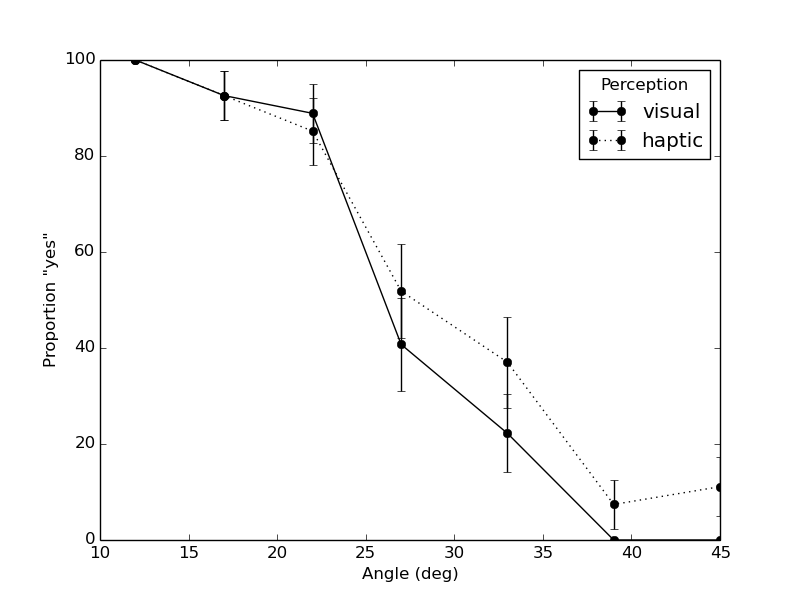
\includegraphics[scale=0.7]{can_step.png}
\caption{\label{fig:pct}Percentage "yes" responses to the question "Does the surface support stable upright posture?" by mode of perception and angle of inclination. Error bars indicate standard error of the mean. Vertical lines indicate the angles resulting in 50\% "yes" responses as estimated by linear interpolation.}
\end{figure}

\begin{figure}
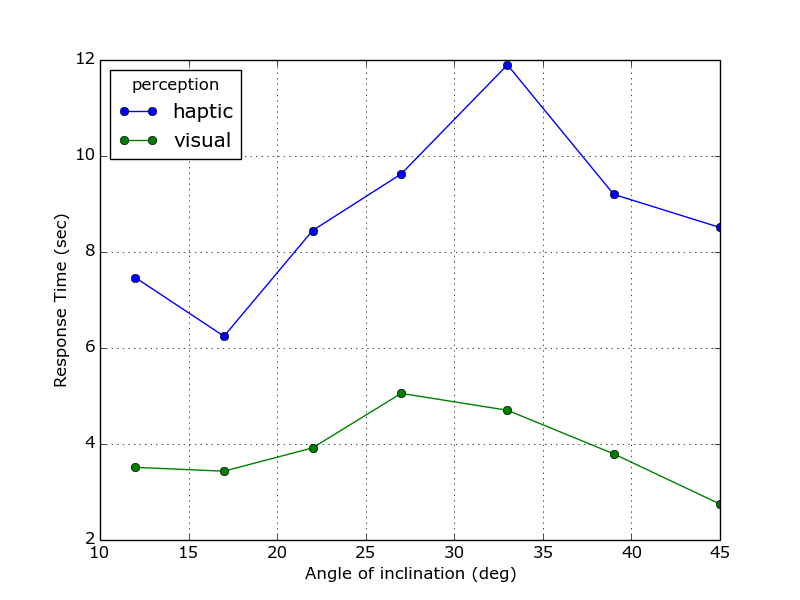
\includegraphics[scale=0.7]{rt.png}
\caption{\label{fig:rt}Average response time by mode of perception and angle of inclination. Error bars indicate standard error of the mean.}
\end{figure}

\begin{figure}
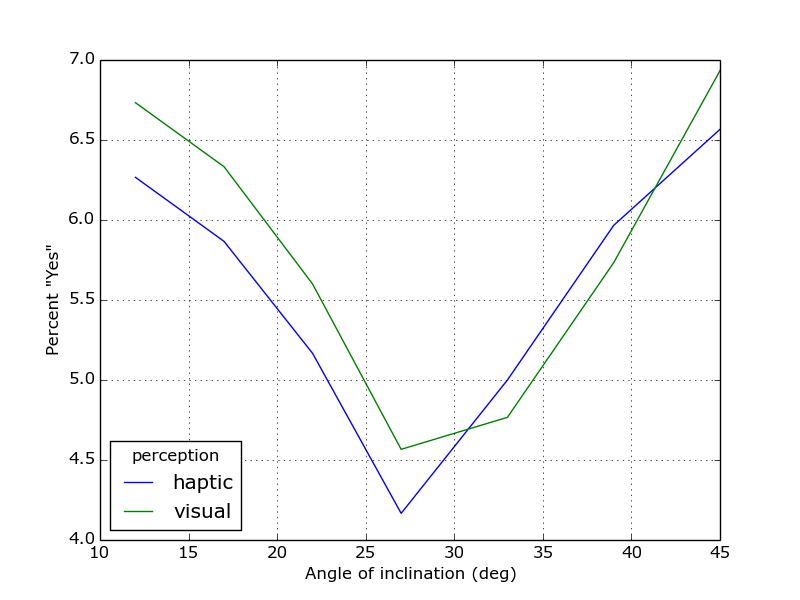
\includegraphics[scale=0.7]{confidence.png}
\caption{\label{fig:confidence}Average confidence judgments, where 1 indicates not confident and 7 indicates very confident, by mode of perception and angle of inclination. Error bars indicate standard error of the mean.}
\end{figure}

\end{document}